This section discusses the results of a rolling window analysis of the parameters from the previous regression models between 
2006 and 2024.
The first subsection compares the rolling window analysis with the Chow test results from Assignment 5.
The following three sections focus on analyzing the parameters (Alpha and Beta), the R-squared and the portfolio,
respectively.

\begin{figure}[h]
    \centering
    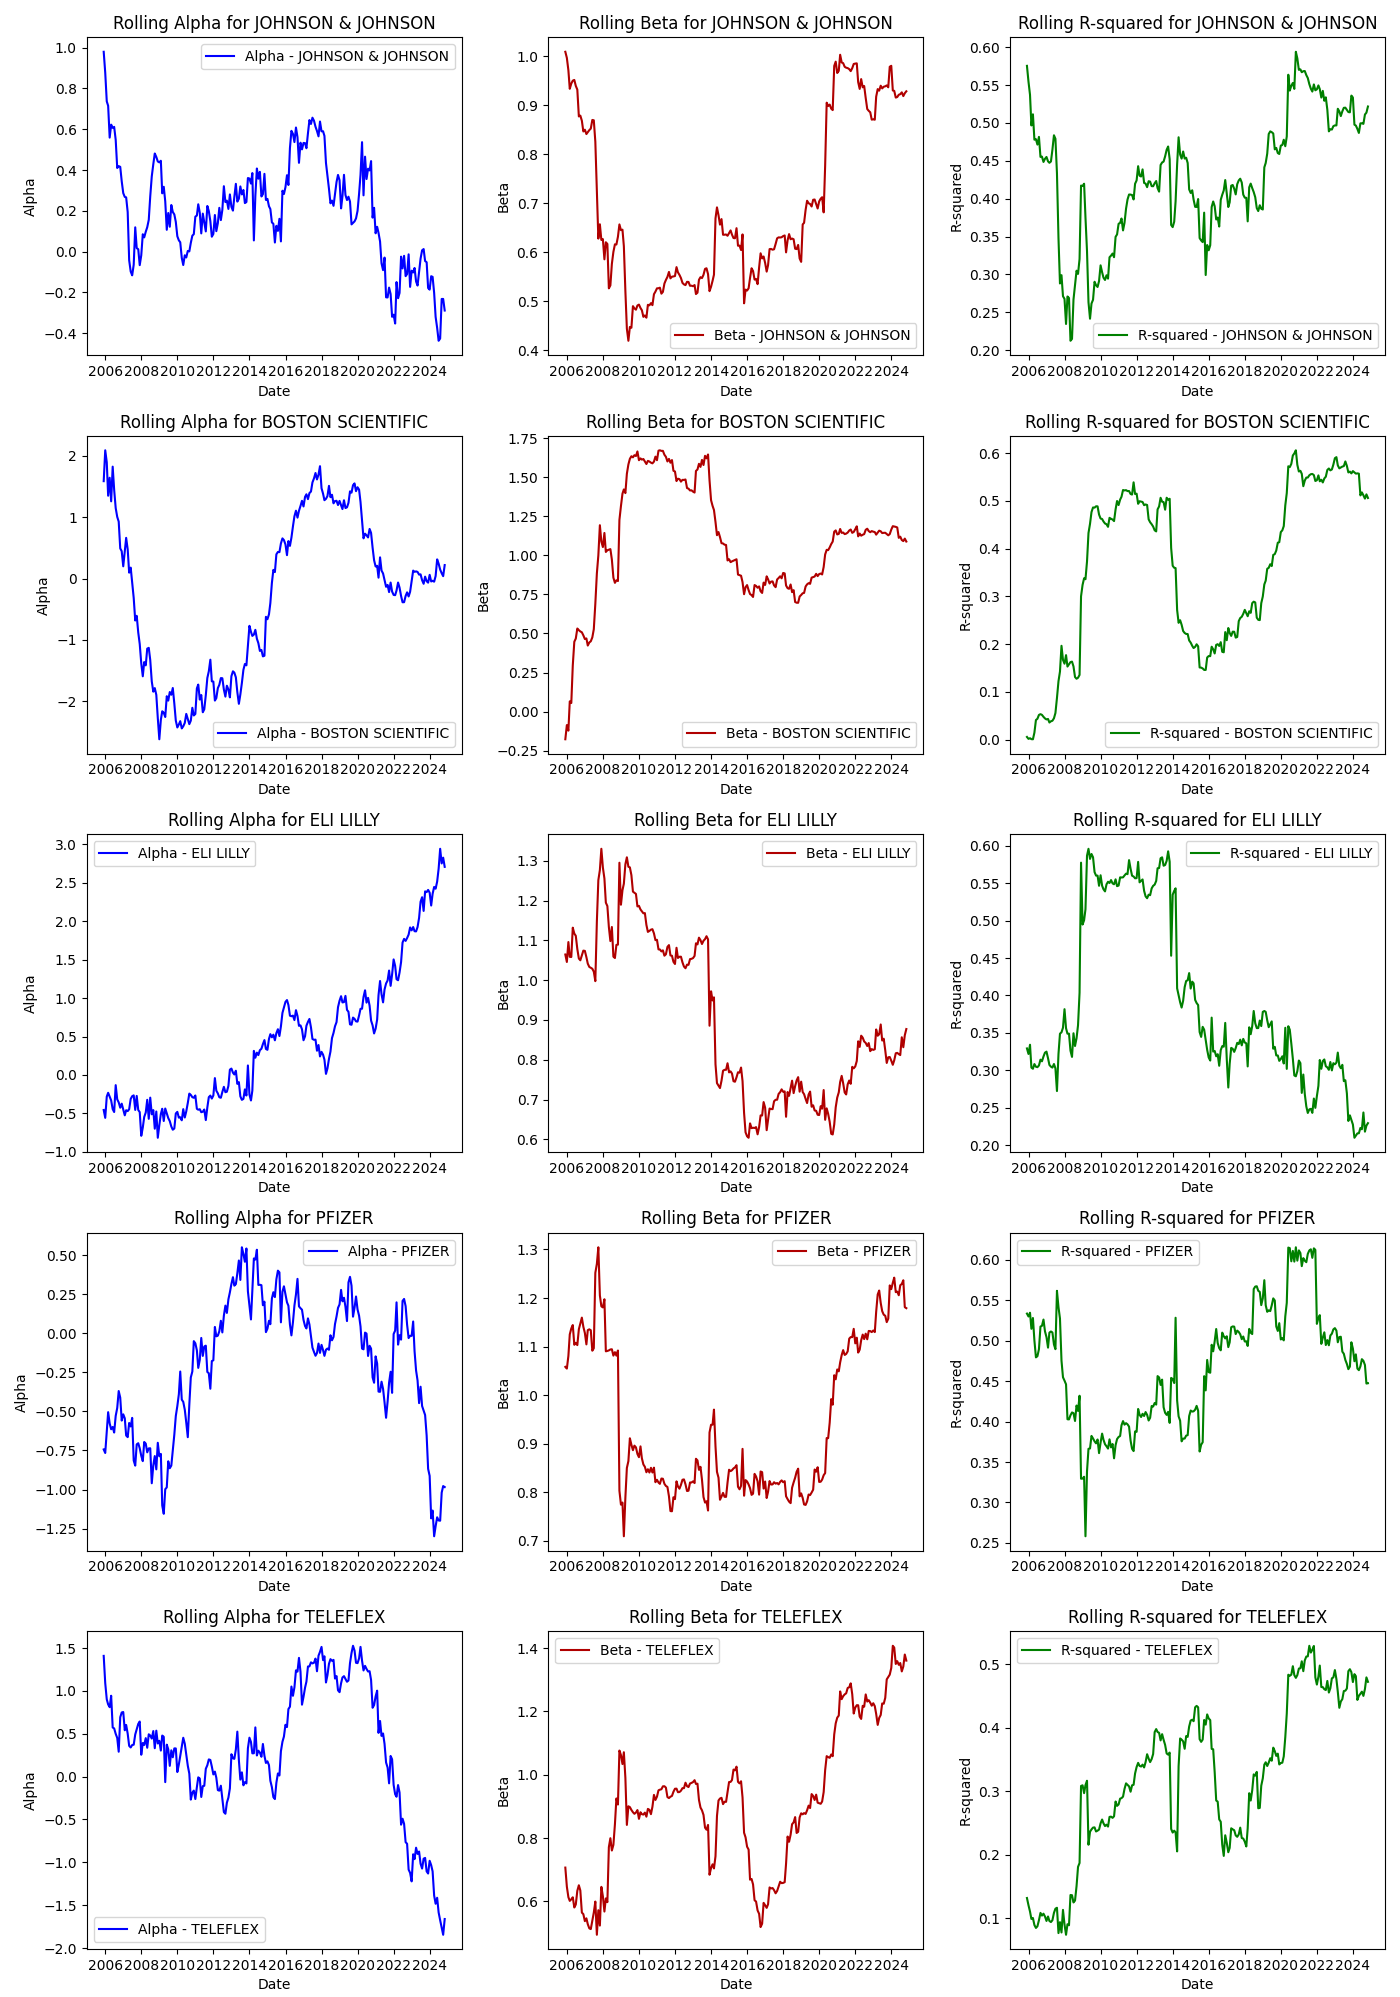
\includegraphics[width=0.8\textwidth]{images/rolling_quantities_1.png}
    \caption{Rolling quantities computed an all equities as an alternative of the Chow Test in search for structural
    breaks (1).}\label{fig:rolling_quantities_1}
\end{figure}
\begin{figure}[h]
    \centering
    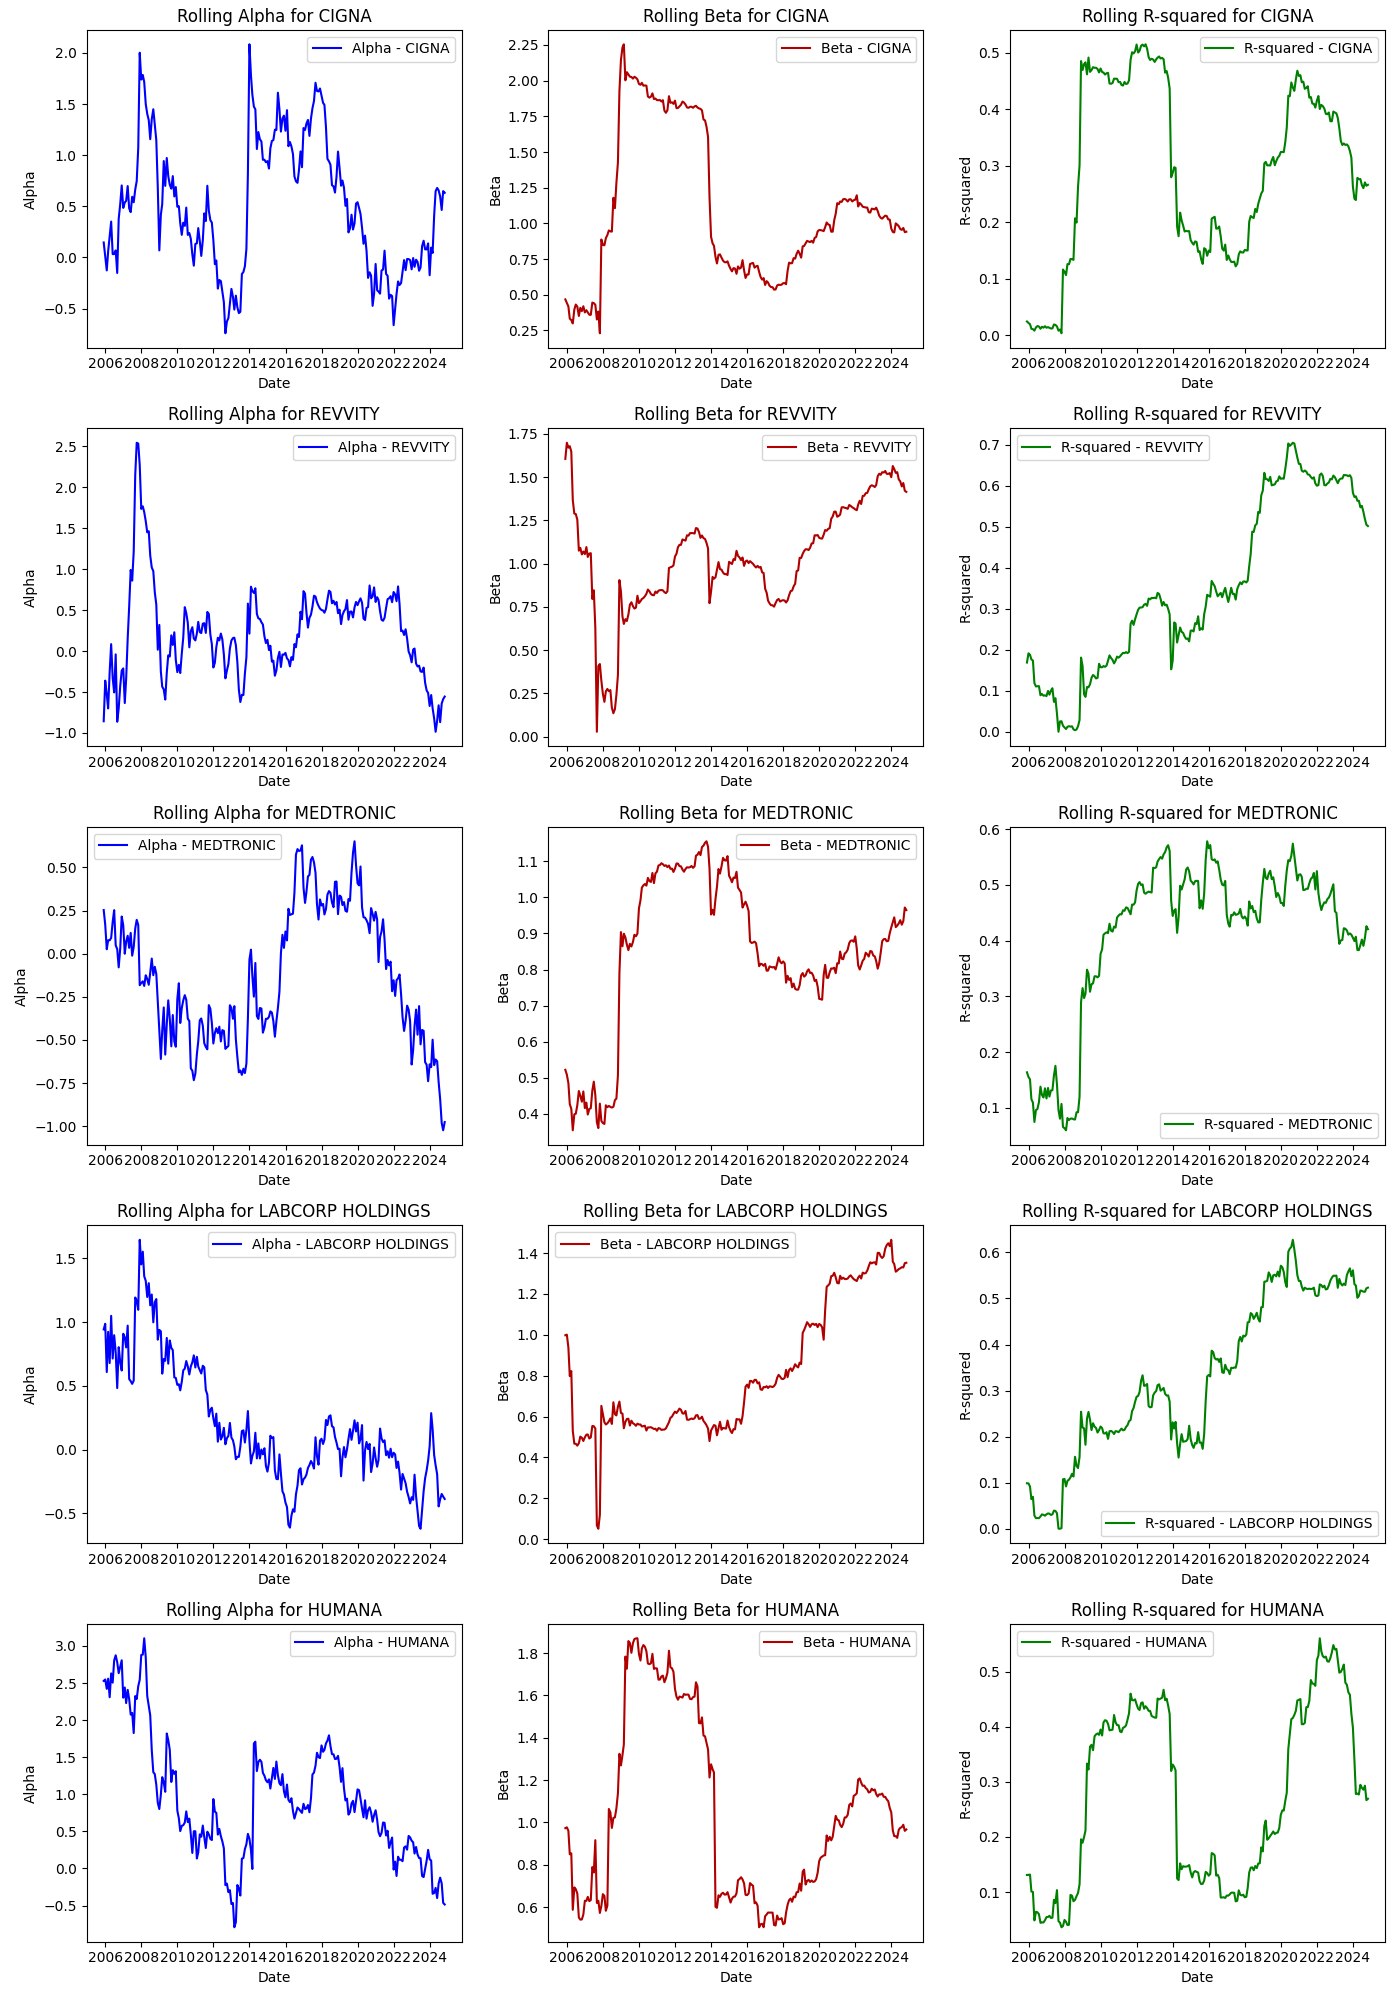
\includegraphics[width=0.8\textwidth]{images/rolling_quantities_2.png}
    \caption{Rolling quantities computed an all equities as an alternative of the Chow Test in search for structural
    breaks (2).}\label{fig:rolling_quantities_2}
\end{figure}

\section{Comparisons with the Chow Test}

The Rolling Window (RW) analysis revealed significant changes in parameters around three key periods: 2008, 2014-2016, and 
2020-2022. These breakpoints likely correspond to major historical events: the subprime mortgage crisis, the implementation of 
the Affordable Care Act (ObamaCare), and the COVID-19 pandemic, respectively.

\subsection{2008}

All regression models had a break date signaled by the RW analysis around the end of 
2008. This is coherent with the results of the Chow test, that indicated structural breaks 
for all stocks in those periods, with the exception of Labcorp Holdings. 
With regards to Labcorp Holdings, the only visible change of its parameter around that 
date is a sharp drop of its Beta, which quickly bounced back to its previous level.  
Apparently the Chow test didn't regard this as a significant parameter change.

%\begin{figure}[h!]
 %   \centering
  %  \includegraphics[width=0.8\textwidth]{images/beta_labcorp.png}
   % \caption{Frequency of months identified as structural break points.}\label{fig:beta_labcorp}
%\end{figure}

\subsection{2014-2016}

In these dates the results of the Chow Test and of the RW analysis are not always linked. 
The RW analysis detected parameter changes for 6 stocks in this period: Johnson \& Johnson, Teleflex, Eli Lilly, Humana,
Boston Scientific and Cigna.
The Chow test, however, failed to detect structural shifts in the parameters of Boston Scientific and Cigna, despite them 
visually indicating important changes.

%\begin{figure}[h!]
 %   \centering
  %  \includegraphics[width=0.8\textwidth]{images/beta_labcorp.png}
   % \caption{Frequency of months identified as structural break points.}\label{fig:beta_labcorp}
%\end{figure}

\subsection{2020-2022}

In this period the RW analysis detected parameter changes for 5 stocks in this period: Johnson \& Johnson, Teleflex, Eli Lilly, 
Labcorp and Pfizer.
Although a few other stocks exhibited parameter shifts during that period, the changes were minimal and insignificant. 
This aligns well with the findings of the Chow test in Assignment~\ref{chapter:chow_test}.

\section{Alpha \& Beta}

The RW analysis is useful not only to detect structural breaks, but it can be useful to analyze the economic meaning of the
parameters too.
Generally speaking, Alphas fluctuated around 0 and Betas fluctuated around a different value for each stock.
There are, however, a few exceptions:
\begin{itemize}
    \item \textbf{Eli Lilly:} Alpha in a constant upward trend and Beta in a downward trend with some fluctuation
    \item \textbf{Boston Scientific:} Beta in an upward trend
    \item \textbf{Medtronic:} Beta in an upward trend with some fluctuation
\end{itemize}

According to the CAPM model and the Efficient Market Theory, the parameter Alpha should be null, since variables are expressed
in excess returns (the risk-free rate is implicit).
\begin{equation}
    r^{e}_{i} = \beta * r^{e}_{m} + \eta
\end{equation}\label{equation:CAPM}

However, when Alpha is different from zero in the regression model it can mean 2 things:
\begin{itemize}
    \item \textbf{Alpha $>$ 0} The stock's returns are beyond what is explained by the industry performance and risk-free rate. 
    It overperforms in relation to its risk.
    \item \textbf{Alpha $<$ 0:} The stock loses value relative to its expected risk adjusted returns. 
    It underperforms in relation to its risk.
\end{itemize}

So, when a stock has its Alpha constantly increasing it may be a signal of the existence of positive external variables that
the market hasn't yet incorporated in the stock's price—market inefficiency. That seems to be the case of Eli Lilly.
The Beta, on the other hand, may assume non null values and still be coherent with the CAPM model. 
From a statistical point of view, Beta represents the sensitivity of a stock's excess returns to the industry's excess returns.
Whereas from an economical point of view Beta measures the sensitivity to systematic risk (economic downturns, interest rate 
changes, geopolitical events).
A changing Beta may be detecting fundamental changes in a company's management strategy or market dynamics such as:
\begin{itemize}
    \item Increase/decrease of leverage
    \item Expanding to more risky or less risky market segments
    \item Mergers \& Acquisitions
\end{itemize}

Therefore, Eli Lilly, Medtronic and Boston Scientific changing Betas are an invitation for further analysis of the companies' 
business models and management strategy.

\section{R-squared}

R-squared measures the strength of the linear relationship between a stock's excess returns and the industry's excess returns. 
In the CAPM framework, Beta represents systematic risk, while the error term reflects idiosyncratic risk-essentially, any
unexplained variance in the model.
A shifting R-squared indicates a change in the relevance of the error term in explaining the dependent variable:

\begin{itemize}
    \item \textbf{Decreasing R-squared:} The error term becomes more significant, suggesting that unknown variables are
    driving the stock's returns.
    \item \textbf{Increasing R-squared:} Beta and industry returns explain the stock's performance more effectively, making it
    more predictable based on systematic factors.
\end{itemize}

Periods of low R-squared may signal market inefficiencies. Investors who identify the specific factors driving a stock's
deviation from market trends can develop strong, informed investment theses. 
Conversely, periods of high R-squared indicate alignment with market trends, where stock-specific opportunities are limited,
and broader market strategies may be more effective.

The R-squared fluctuated throughout the study period (2006-2024), with notable variations in 2008 and 2020, both periods of 
high systemic risk—the subprime crisis and COVID-19 pandemic.
In 2008, R-squared behaved differently across stocks: it increased for some, indicating stronger ties to market trends and
greater impact from the crisis, while it decreased for others, suggesting weaker market influence.
In contrast, 2020 saw R-squared increase for all analyzed stocks, highlighting COVID-19 as a major systemic risk that 
significantly explained returns across the board.

\section{The portfolio}
The portfolio's Beta and Alpha visually signal 3 possible structural break periods, 2008, 2016 and 2020.
 
This result does not entirely align with the Chow test, as no structural break was identified in 2020.
Despite relatively high R-squared values (ranging from 0.65 to 0.85), the data displays trends similar to stock movements, 
characterized by notable fluctuations.
Three significant changes stand out:
\begin{itemize}
    \item \textbf{2008:} A sharp decline followed by a quick recovery.
    \item \textbf{2014:} A marked drop.
    \item \textbf{2020:} A drastic increase.
\end{itemize}